\section{Vorwort}
Die Dokumentation orientiert sich an der Reihenfolge der Aufgaben im Bewertungsschema.
Alle Testprogramme funktionieren und die Hardwareansteuerung wurde umgesetzt.



\section{Simulatoren}
Entwickelt wurde ein Simulator für den PIC16F84:
Also eine Software, die das Verhalten dieses Mikrocontrollers nachbildet,
um PIC16F84 Assemblerprogramme auf einem x86 Computer in einer grafischen Oberfläche Ausführen zu können.
Hierbei wurde nicht das genaue Verhalten implementiert, mit allen internen Zuständen,
sondern das Ergebnis nach außen.



\section{Funktionsweise}

\subsection{Gewählte Technologien}
Die Software ist als Webanwendung umgesetzt.
Es gibt also zwei Teile, in die die Anwendung unterteilt werden kann:
Front- und Back-End.
Das Back-End ist in der Programmiersprache C\# geschrieben, mit der \char`\~90~\% des Codes geschrieben wurde.
Die Logik im Front-End in JavaScript.
Zum Beschreiben der grafischen Oberfläche wird HTML verwendet.
Es wird das Blazor\urlfootnote{https://dotnet.microsoft.com/en-us/apps/aspnet/web-apps/blazor} Web-Framework verwendet.
Der Grund für die Wahl von Blazor ist,
diese (für uns unbekannte Technologie) beim Entwickeln dieses Projekts kennenzulernen. 


\subsection{Einlesen von Programmen}
Das Einlesen der LST-Dateien funktioniert über einen Parser im Front-End,
der mit dem Parsergenerator Tree-sitter\urlfootnote{https://tree-sitter.github.io/tree-sitter/} erstellt wurde.
Tree-sitter generiert aus einer LR(1) Grammatik C-Code für einen Parser,
der zu WebAssembly kompiliert wird, ein Bytecode-Standard der W3C zum Ausführen von Programmen innerhalb des Webbrowsers.
Die Anbindung an die JS-API des Browsers funktioniert über eine 
Bibliothek\urlfootnote{https://github.com/tree-sitter/tree-sitter/tree/master/lib/binding_web} des Tree-sitter Projekts.
Das ist der Grund dafür, dass dieser Teil der Logik im Front-End ist.

\js[Auszug der Grammatik für LST-Dateien (\texttt{tree-sitter-pic/grammar.js}).]{./listings/grammatik.js}

Der Parser baut einen konkreten Syntaxbaum auf.
Durch Traversieren des Baumes wird der LST-Text (zum Anzeigen mit Syntaxhervorhebung) in HTML-Elemente verpackt,
weiter werden durch das Traversieren die relevanten Informationen für den Simulator extrahiert:

\begin{itemize}
    \item Position im Programmspeicher
    \item Opcode 
    \item Zeilennummer im Quellcode (für Breakpoints)
\end{itemize}

Diese Informationen werden an das Back-End (den C\# Teil) übergeben,
der damit ein \texttt{Pic}-Objekt initialisiert, das Hauptobjekt des Simulators.

\subsection{\texttt{Pic}-Objekt}
Das Hauptobjekt im Simulator im vom Typt \texttt{Pic}.
Es enthält alle simulierten Elemente des PIC16F84,
wie z. B. den Hauptspeicher, Programmspeicher und das W-Register. 


\subsection{Befehle}

\subsubsection{Befehlsdecodierung}
Die Befehlsdecodierung funktioniert über das Interpretieren der geparsten Opcode-Zeichenketten als Zahlen.
Diese werden wieder als Strings dargestellt mit Binärdarstellung (der Zahlen),
für einen Vergleich vom Stringanfang, um den Befehl zu bestimmen.

\cs[Logik zum Decodieren der Opcode-Strings (\texttt{Simulation/InstructionDecoder.cs}).]{./listings/instruction-decoder.lst}

\subsubsection{Befehlsmodellierung}
Befehle werden durch Klassen modelliert (z. B. \texttt{ADDWF}).
Sie erben alle von der abstrakten Klasse \texttt{Instruction}.

\paragraph{Programmspeicher}
Der Programmspeicher ist ein Array vom Typ \texttt{Instruction},
das alle decodierten Befehle in Reihenfolge der LST-Datei enthält. 

\texttt{Instruction}-Objekte haben eine Referenz auf ihr zugehöriges \texttt{Pic}-Objekt
und verändern durch Aufruf ihrer \texttt{Execute}-Methode den Zustand von diesem;
z. B. die Flags im Statusregister.

\cs[\texttt{Execute}-Methode vom MOVLW-Befehl (\texttt{Simulation/Instructions/LiteralInstructions/MOVLW.cs})]{./listings/movlw.lst}

\paragraph{Befehlsabarbeitung}
Die Befehlsabarbeitung funktioniert über eine Schleife,
die mit dem Programmzähler (als Index) den aktuellen Befehl aus dem Programmspeicher-Array holt.
In dieser Schleife werden auch die Cycles gezählt.
Zwei Cycle Anweisungen werden beachtet.
Die Cycles werden mit der einstellbaren Frequenz für die Laufzeitberechnung verwendet. 


\subsection{Hauptspeicher}
Der Hauptspeicher ist als Klasse \texttt{Memory} umgesetzt,
die ein Array vom Typ \texttt{uint} für die Register enthält.
Das Lesen und Schreiben in den Hauptspeicher funktioniert über spezielle Methoden: \texttt{ReadRegister} und \texttt{WriteRegsiter}.
In diesen Methoden werden Bedingungen wie die Adressspiegelung für spezielle Register umgesetzt.

\cs[Teil der Switch-Case in der \texttt{WriteRegister}-Methode]{./listings/switch-case-memory.lst}

Weiter gibt es zwei extra Methoden für das Lesen und Schreiben,
die das \texttt{RP0}-Bit beachten. 


\subsection{Programmzähler}
Der Programmzähler wird in der Variable \texttt{\_programCounter} in \texttt{Pic} gespeichert.
Das Schreiben funktioniert über einen Setter,
der immer das Pcl-Regsiter aktualisiert.
Falls in das Pcl-Register geschrieben wird,
wird die \_programCounter Variable aktualisiert (von der \texttt{Memory}-Klasse aus).

\paragraph{PCLATH}
Der Wert im PCLATH-Register wird bei jedem \texttt{GOTO} und \texttt{CALL} Befehl beachtet.
Hier wird in der \texttt{Execute}-Methode die \texttt{\_programCounter} Variable aktualisiert.
Die Beachtung für z. B. ein \texttt{ADDWF} wird auch in der \texttt{Memory}-Klasse umgesetzt,
wenn in das PCL-Register geschrieben wird. 


\subsection{Timerfunktion}
Der Timer wurde zum Teil in der Pic Klasse und zum Teil in der PortA Klasse realisiert.  Zunächst musste eine Prescaler Variable erstellt werden, welche sich der Timer und Watchdog teilen. Hierzu wurde zunächst eine Art decoder Funktion mit dem Namen GetScalerRate() erstellt. Diese Wertet automatisch die Werte welche in PS0, PS1, PS2 und PSA stehen aus und gibt den entsprechenden Wert für den Prescaler zurück. Immer wenn die Simulation einen Cycle ausführt, wird das T0CS Bit überprüft und gegebenenfalls die TimerStep() Funktion aufgerufen. Diese wiederrum überprüft anhand des PSA -Bit ob der Timer den Prescaler zugewiesen hat oder nicht. Wenn der Timer den Prescaler zugewiesen hat, so wird dieser zunächst dekrementiert, bis dieser den Wert 0 erreicht. Danach wird der Prescaler zurückgesetzt und die Funktion IncreaseTimer() aufgerufen. Sollte der Prescaler nicht dem Timer zugewiesen sein wird diese Methode sofort aufgerufen. IncreaseTimer() holt sich zunächst den aktuellen Wert aus dem Speicher des Pics. Danach wird dieser inkrementiert und es wird überprüft, ob es einen Überlauf gab. Ist dies gegeben, so wird der Timerwert auf die untersten 8 Bit maskiert. Außerdem wird überprüft, ob der Timer0 Interrupt aktiv ist durch das Bit T01E. Ist auch dies gegeben wird die Interrupt Routine, also Interrupt(), ausgelöst und das entsprechende Flag in T0IF gesetzt. Unabhängig davon, ob es einen überlauf gab oder nicht, wird der neue Timer-Wert wieder in den Speicher des Pics geschrieben. Natürlich werden die aktuellen Werte des Prescalers und des Timers auch noch in der UI angezeigt. Unabhängig von all dem wird in der PortA Klasse beim togglen des RA4 Pins über das T0CS Bit geprüft, ob RA4 als Clock Source verwendet wird. Ist dies der Fall so wird über das T0SE Bit geprüft, ob es sich um eine steigende oder eine fallende Flanke handeln soll. Demensprechend wird dort ebenfalls die TimerStep() Funktion des Pics aufgerufen.


\subsection{Interrupts}
Abgesehen von dem gerade beschriebenen Timer Interrupts gibt es noch 3 weitere Interrupts. 
Zunächst gibt es noch den EEPROM Interrupt. Dieser ist implementiert, indem am Ende des EEPROM Schreibvorganges das entsprechende EEIE Bit überprüft und gegebenenfalls die Interrupt() Methode aufgerufen wird. 
Weiterhin gibt es den RB0/INT Interrupt. Hierbei wird bei einem Toggle an RB0 zunächst durch das INTE Bit überprüft, ob dieser aktiv ist. Danach wird über das NTEDG Bit der Flankenmodus ausgelesen. Danach wird überprüft ob die aktuelle Flanke dieser entspricht und gegebenenfalls die Interrupt() Methode aufgerufen. Außerdem wird das INTF Flag gesetzt, um zu signalisieren um welche Art von Interrupt es sich handelt.

Dasselbe wird auch bei den Pins RB4-7 getan jedoch ohne die Selektierung der Flanke. Hier wird jedoch das RBIF Bit als Flag gesetzt.

Die Interrupt() Methode pusht zunächst den aktuellen Programcounter wert auf den Stack und setzt ihn dann auf den Wert 4. Im Falle das der Pic Schläft werden stattdessen das TO und PD Bit entsprechend gesetzt und die IsSleeping Variable auf false gesetzt.

\subsection{Sleep}
Sleep wurde zunächst anhand von der Dokumentation implementiert, um die Entsprechenden Bits in den Registern zu setzen. Zusätzlich wird noch die interne Variable des Pics mit dem Namen IsSleeping gesetzt. In der Step() Funktion des Pics wird diese Variable überprüft und nur falls der Pic nicht schläft wird die nächste Instruction ausgeführt. Die IsSleeping Variable kann nur durch einen Interrupt oder einen Reset wieder auf false gesetzt werden.


\subsection{Watchdog}
Der Watchdog hat eine eigene wdtCheck() Funktion in der Pic Klasse welche wie die Cycle() Methode beim durchlauf jedes Steps ausgerufen wird. Während in der Cycle() Methode die entsprechende Zählvariable des Watchdos hochgezählt wird, überprüft die wdtCheck() Methode nur ob die Laufzeitsumme der bisherigen Cycles einen Wert über 18ms ergibt. Ist dies der Fall wird über das PSA Bit überprüft, ob der Watchdog den Prescaler zugewiesen bekommen hat. Ist dies der Fall wird dieser dekrementiert. Sobald dieser den Wert 0 erreicht oder falls der Prescaler nicht dem Watchdog zugewiesen ist, wird die WatchDogReset() Methode aufgerufen.
Die WatchDogReset() Methode überprüft zunächst, ob der Pic schläft. In diesem Fall wird der Pic aufgeweckt, das PD und TO Bit entsprechend gesetzt und der Programcounter inkrementiert. Schläft der Pic nicht so wird stattdessen ein Reset ausgeführt und mögliche EEPROM Schreibvorgänge werden terminiert.


\subsection{EEPROM}
Die EEPROM wird mit der Klasse \texttt{EEPROM} dargestellt.
Wie bei \texttt{Memory} sind die Speicherstellen über ein \texttt{uint}-Array abgebildet.
Das Lesen aus \texttt{EEPROM} wird bei jedem setzen des Read Control Bits (im \texttt{EECON}-Register) ausgelöst.

\paragraph{Lesen}
Das Prüfen erfolgt über die Akzessoren für das {EECON}-Register in der \texttt{EEPROM} Klasse,
die von der Klasse \texttt{Memory} immer verwendet werden, wenn auf das Register zugegriffen wird.

\paragraph{Schreiben}
Das Schreiben wird ähnlich wie das Lesen über das \enquote{Write Control Bit} ausgelöst.
Zusätzlich muss eine \enquote{write sequence} davor erfolgt sein.
In dieser Implementierung löst das Setzen des \enquote{Write Control Bit} nur direkt nach der \enquote{write sequence} ein Schreiben aus.
Die Prüfung für diese Bedingung erfolgt in der Schleife für die Befehlsabarbeitung.
In der Schleife wird immer \texttt{EEPROM.CheckInstruction} Methode aufgerufen.

\cs[Code zum Prüfen der \enquote{write sequence}]{./listings/eeprom.lst}

Die Bedingung zum Auslösen des Schreibens entspricht damit \texttt{\_nextRequiredInstructionForWrite == 4}.


\paragraph{Programmierzeit}
Die Programmierzeit wird sehr einfach über die Laufzeitberechnung umgesetzt.
Wenn geschrieben wird, wird die aktuelle Laufzeit in einer Variable gespeichert.
In der Befehlsabarbeitungsschleife wird geprüft,
ob die Differenz zwischen aktueller und gespeicherter Laufzeit größer gleich 1~ms ist. 


\subsection{I/O Ausgangslatch}
Die Wirkung des Ausgangslatch wird in der Klasse \texttt{Port} umgesetzt.
Sie bietet Akzessoren für einen internen Zustand,
der dem Zustand widerspiegelt der per Software (im Assembler-Code) gelesen wird
und einem externen Zustand,
der dem physikalischen Wert am Pin entspricht.
Der \enquote{physikalische} Zustand der Pins wird in einer extra Variable gespeichert.


\paragraph{TRIS Output}
Wenn im Tris-Register ein Pin auf Output eingestellt ist,
sind interner und externer Zustand gleich.
Bei jedem Aufruf eines Akzessor wird für Output-Pins der Wert im Port-Register auf die Pin-Variable (\enquote{physikalisch}) geschrieben.
So wird bei einem Umschalten auf Output auch direkt der Wert im Register auf die Pins ausgegeben.  


\paragraph{TRIS Input}
Für einen Pin im Input Modus löst das Setzten eines Werts über den Akzessor für den internen Zustand – ein Schreiben auf das Port-Register aus.
Gelesen wird jedoch immer von der Variable für den physikalischen Zustand (Pin).
Das Setzen über den Akzessor für den externen Zustand verwendet genau diese.


\subsection{Hardwareanbindung}
Zur Hardware Anbindung wird nach jedem Cycle die Methode serialHandler.Write() aufgerufen. Der Serialhandler baut über die aus der Doku gegebenen Parameter (Baudrate 4800, Parity None, Databits 8, Stopbits 1) eine Verbindung zur externen Hardware auf. Der Write Methode wird ein zuvor per GenerateSerialPayload() generiertes Payload übergeben. Das Payloud besteht entsprechend der Doku aus High- und Lowbytes des Tris A/B und Port A/B Registers und wird mit einem CarriageReturn abgeschlossen. Nachdem das Payload abgeschickt wurde, wird überprüft, ob eine mindestens 5 Byte lange Antwort entgegenkam. Falls dies der Fall ist, werden die Halbbytes wieder zu vollen Bytes verknüpft und die entsprechenden Register geschrieben.


\section{Zusammenfassung}

\subsection{Ergebnis}
Das Ergebnis dieses Projekts ist ein Simulator,
der jedes Testprogramm korrekt ausführen kann.
Über die grafische Oberfläche wird jeder Zustand,
die der Nutzer am PIC16F84 nachvollziehen kann angezeigt.
Verhalten wie der \enquote{weak pull-up} an \texttt{PPORTB} Pins wurden nicht per Software nachgebaut.

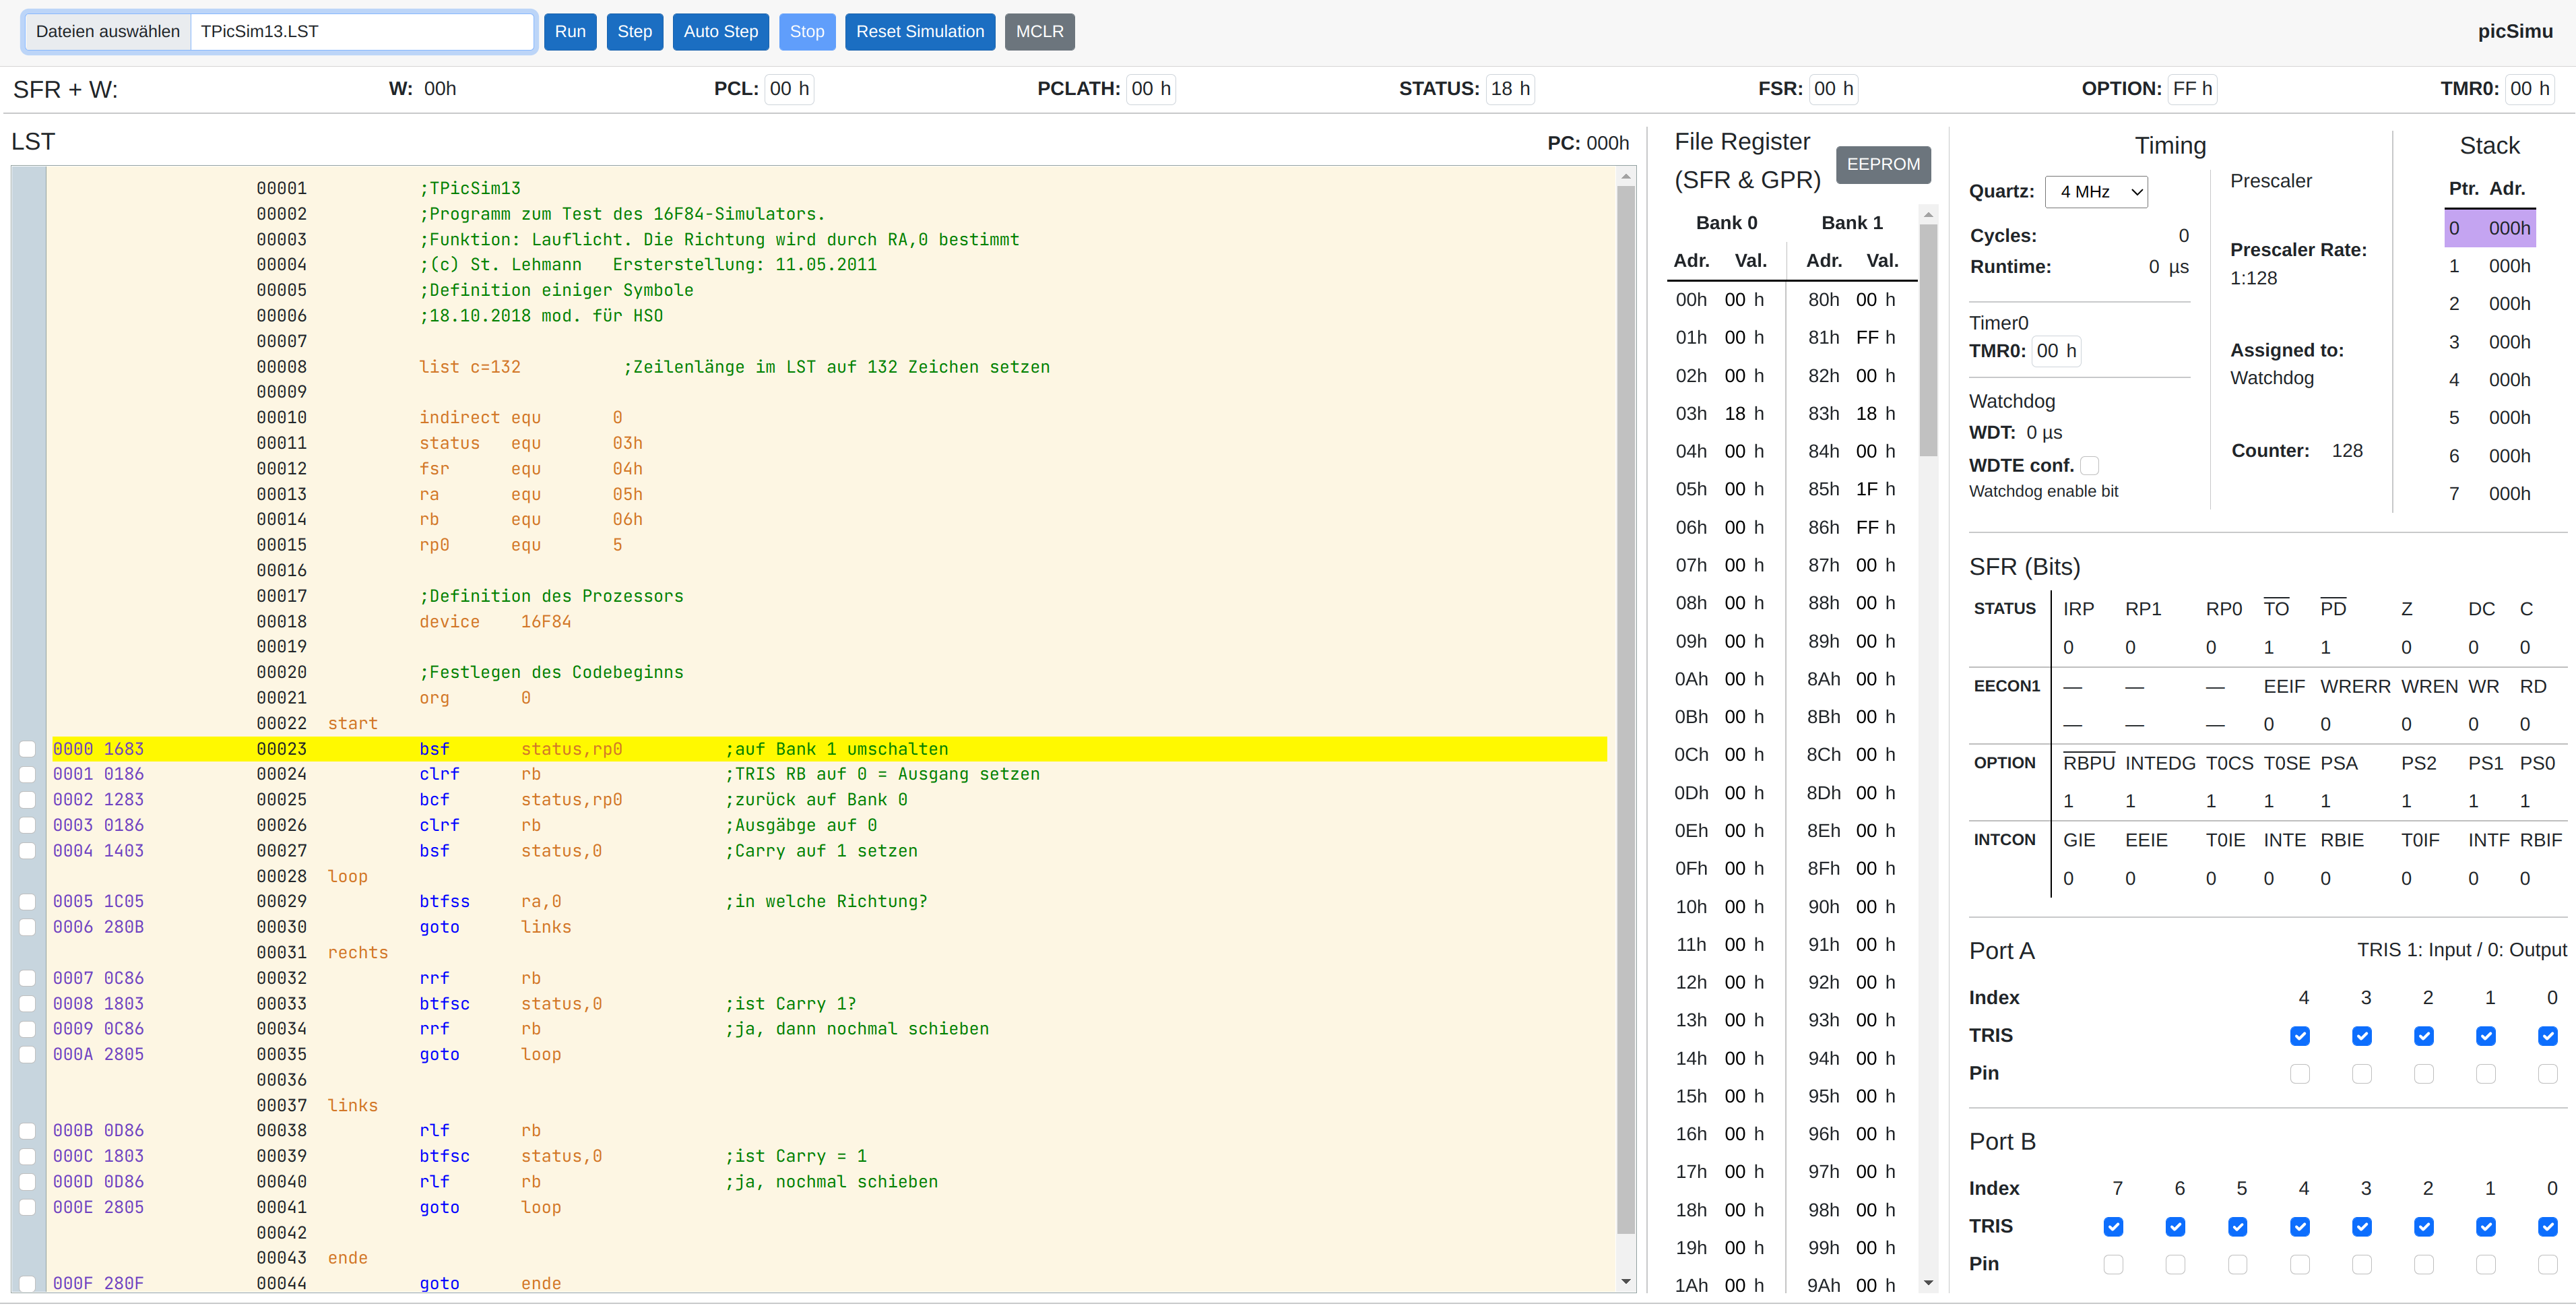
\includegraphics[width=\textwidth]{gui.png}

Erwähnenswert ist, dass der Simulator auch komplett ohne Server lauffähig ist (als standalone WebAssembly),
wenn das Projekt entsprechend kompiliert wird.


\subsection{Persönliches Fazit (Valerio Cocco)}
Die Entwicklung am Simulator hat mir persönlich gut gefallen.
Zuvor habe ich nichts Vergleichbares programmiert.
Durch dieses Projekt konnte ich mein Verständnis über die Arbeitsweise von Mikrocontrollern und damit Computern verbessern und festigen.

Weiter ist mir noch mal klar geworden,
dass Computer aus einer sehr abstrakten Sichtweise als Zustandsautomat betrachtet werden können.
In diesem Fall der Pic mit all seinen Komponenten, die den Zustand widerspiegeln (Register, Timer, Watchdoch, usw.)
und
Bedingungen/Eingaben wie, Zyklen, Befehle, Pin Signale, etc. die Zustandsänderungen bewirken.

Besonders interessant/neu für mich war der sehr hardwarenahe Teil wie Interrupts, Data Latches und EEPROM-Programmierzeit.

Neben diesen Aspekten habe ich auch viel über die verwendeten Werkzeuge wie C\# und Blazor gelernt.

Mit der Zusammenarbeit zwischen meinem Partner und mir, bin ich sehr zufrieden.
Wir konnten die Aufgaben gut aufteilen, selbstständig arbeiten,
fertiggestellte Teile zusammen besprechen und uns bei Problemen gegenseitig unterstützen.

Der zeitliche Umfang des Projekts war sehr groß.
Tatsächlich hätten wir auch Aufgaben weglassen können für eine 1,0.
Ich denke aber, die Tatsache, dass wir alle Aufgaben umgesetzt haben,
zeigt, dass wir nicht ungern am Projekt gearbeitet haben.
Für das nächste Mal nehme ich mir vor mich auf die wichtigsten Aspekte eines solchen Projekts zu fokussieren, um Zeit zu sparen.
Z. B. hätte ich Angelegenheiten wie das Aussehen der Benutzeroberfläche weiter hinten anstellen können.  



\subsection{Persönliches Fazit (Daniel Rittershofer)}
Ich persönlich finde das Projekt eine sehr gute Aufgabe, um die internen Funktionsabläufe und das Arbeiten des besser zu verstehen. Durch das Projekt habe ich nicht nur gelernt wie die einzelnen Befehle, welche der PIC beherrscht funktionieren, sondern auch, wie der PIC Interrupts und Timer realisiert und handhabt. Zu Beginn des Projekts war mir noch gar nicht so richtig klar, was wir alles benötigen, um den PIC vollständig zu simulieren aber durch die Aufeinander aufbauenden Aufgaben konnte unser Projekt immer um die fehlenden Bausteine erweitert werden. Beispielsweise der Stack, welcher als Ringspeicher realisiert werden musste. Für die ersten Programme konnte dieser ignoriert werden, doch als er dann benötigt wurde konnten wir mithilfe eines selbst erstellen RingBuffer Datentyps, da C\# diesen Datentyp nicht bereitstellt, einfach realisieren und einbauen.  Ebenfalls hilfreich fand ich es, dass einem im Laufe der Programme neue Fehler auffallen, welche man zuvor übersehen hat. Beispielsweise haben wir uns Anfangs keine größeren Gedanken gemacht, was passiert, wenn es einen Overflow beim addieren oder anderen Operationen gibt. Erst als es bei einem Programm zu einem überlauf kam und das erwartete Ergebnis nicht übereinstimmte fiel uns dies auf und wir konnten es durch eine Maskierung auf die niedrigsten 8 Bit beheben. Beim Nächsten mal eines solchen Projekts würde ich nicht viel verändern, da ich sehr zufrieden mit unserem Endergebnis und unseren Arbeitsprozessen war. Lediglich zu Beginn des Projekts würde ich mehr Zeit in einen genaueren Plan investieren.

